\newpage
\rhead{\textbf{\textcolor{blue}{О}\textcolor{gray}{пределение термина «информатика» }}}
\makebox[0pt][l]{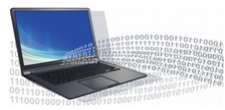
\includegraphics[scale=0.5]{img/pic.png} }
\vspace*{4mm}
\newline
\textcolor{Green}{Информатика}
– дисциплина, изучающая свойства и структуру информации,
закономерности ее создания, преобразования, накопления, передачи и
использования.

\vspace*{1mm}
\textcolor{Green}{Англ}
: informatics = information technology + computer science + information
theory

\vspace*{2mm}
\begin{center}
  \textbf{Важные даты}
\end{center}
			\textbullet \ 1956 – появление термина «информатика» (нем. Informatik, Штейнбух) \\
			\textbullet \ 1968 – первое упоминание в СССР (информология, Харкевич) \\
			\textbullet \ 197Х – информатика стала отдельной наукой \\
			\textbullet \ 4 декабря – день российской информатики